% kapitel2.tex
\chapter{Implemented Changes}
\label{chapter:implementedChanges}

This work extends Tour4Me\footnote{\url{http://tour4me.cs.tu-dortmund.de/}}, which is an application written in C++, HTML and JavaScript. 
The implemented interface of this extension uses C\# as programming language to enable easy porting of the web application to a desktop or mobile application.
To improve the query times and allow for easier coverage of the whole world (see \ref{sec:futureWork}), a database that offers features of a spacial database was added. 
Reasons for and positive effects of this decision are described in the following section.

Furthermore, not only the language and data access was changed.
New options and parameters to improve the customizability of preferences for a generated tour were added as well.
These changes had to be incorporated into an upgraded front end design (see sections \ref{subsec:interfaceAndFrontendChanges} and \ref{sec:parameterChanges}) as well as into the back end and all solvers (see section \ref{sec:algorithmicChanges}). 


\section{Application}
\label{sec:application}

To include the various changes, the whole application -- including the front end representation, the back end implementation and the data retrieval -- was changed.
The Open Street Map (OSM) data are downloaded and stored in a database from which the graph for calculating the roundtrips is build.
Furthermore, the design of the front end was changed to improve the overview and general user experience as well as to allow for the addition of new customization options.
Lastly, the algorithms to choose from have been extended by two additional meta-heuristic approaches.

\subsection{New Architecture}
\label{sec:newArchitecture}

For the new application, the architecture had to be re-structured.
An illustration of the new design is shown in figure \ref{fig:architecture}.
Instead of reading the data for the graph from a static \textit{.txt} file, which contains all the nodes and edges for Dortmund, a database is used to manage the nodes, edges, their additional information and the relationships between them. 
It can be filled with the data needed by using an import python script that creates an osmnx-graph\footnote{\url{https://osmnx.readthedocs.io/en/stable/}, last accessed: 15.04.2024}\footnote{\url{https://networkx.org/}, last accessed: 22.03.2024}\footnote{\url{https://wiki.openstreetmap.org}, last accessed: 22.03.2024}\footnote{\url{https://wiki.openstreetmap.org/wiki/Main_Page}, last accessed: 19.04.2024} for a user specified location. 
From this graph, the nodes and edges can be extracted alongside their additional information.
For the current use case, nodes are stored with their OSM-ID, which is transformed into a UUID, their latitude and longitude coordinates as well as their elevation profile and tags of the surroundings they are placed in.
The elevation data has to be acquired from a different source than OSM, since they do not use a height profile. 
A few open source providers were available, but ultimately, Open-Elevation\footnote{\url{https://open-elevation.com/}, last accessed: 20.03.2024} was used. 

Since most open source providers have a limited bandwidth to supply users with data based on their API-calls, the opportunity to use a locally hosted version that Open-Elevation offered was very important to assure usability.
When using the python script to create and fill the database and its tables, the Open-Elevation data needs to be available.
A local docker container with the respective data can be used to access the needed information without being bound to the servers and their throughput boundaries. 
Even though the accuracy of the version that can be hosted locally is not ideal, it was the easiest method that did not rely on querying a website and being limited by their API-call restrictions.
In the section future work (\ref{sec:futureWork}), a few other options of including other data sources are discussed.

The used database is Microsoft SQL Server Management Studio\footnote{\url{https://learn.microsoft.com/en-us/sql/sql-server/sql-docs-navigation-guide?view=sql-server-ver16}, last accessed: 22.03.2024}, which can handle spatial data, supports spatial queries and works well in combination with the C\# implementation.

The back end is implemented in C\#\footnote{\url{https://learn.microsoft.com/en-us/dotnet/csharp/}, last accessed: 22.03.2024}, as this language allows for the opportunity to also create a mobile- or desktop application in addition to the web application that already exists (see \ref{sec:futureWork}).
Furthermore, C\# allows for using SQL queries and filtering using LINQ for easy runtime database querying\footnote{\url{https://docs.telerik.com/devtools/aspnet-ajax/controls/grid/asp.net-3.5-features/linq-to-sql---binding-and-automatic-crud-operations}, last accessed: 22.03.2024}.
Here, the Tour4Me application was automatically translated from C++ to C\# using ChatGPT. 
This translation is not part of the thesis and only allows for easier extension, since the basic structures that are used in Tour4Me did not need to be re-implemented from scratch.


The front end is implemented using HTML\footnote{\url{https://devdocs.io/html/}, last accessed: 22.03.2024}, CSS\footnote{\url{https://devdocs.io/css/}, last accessed: 22.03.2024}, JavaScript\footnote{\url{https://devdocs.io/javascript/}, last accessed: 22.03.2024} and C\# code behind. 
The base-styling is done using bootstrap\footnote{\url{https://getbootstrap.com/docs/4.3/getting-started/introduction/}, last accessed: 22.03.2024}, but additional custom CSS is added to create a nature-based color palette (\#TODO references to color theory stuff?) as well as several custom effects and transitions for the side and bottom menus.
To realize the communication between front end and back end, Ajax-queries\footnote{\url{https://api.jquery.com/category/ajax/}. last accessed: 22.03.2024} are used.

The map is a leaflet\footnote{\url{https://leafletjs.com/}, last accessed: 20.03.2024} visualization that shows Open Street Map data.
The leaflet map allows to set markers, add a search bar, create polygons - which are used to illustrate the generated routes - and offers an open source map view. 


\begin{figure}[ht]
	\hspace*{-25 pt}
	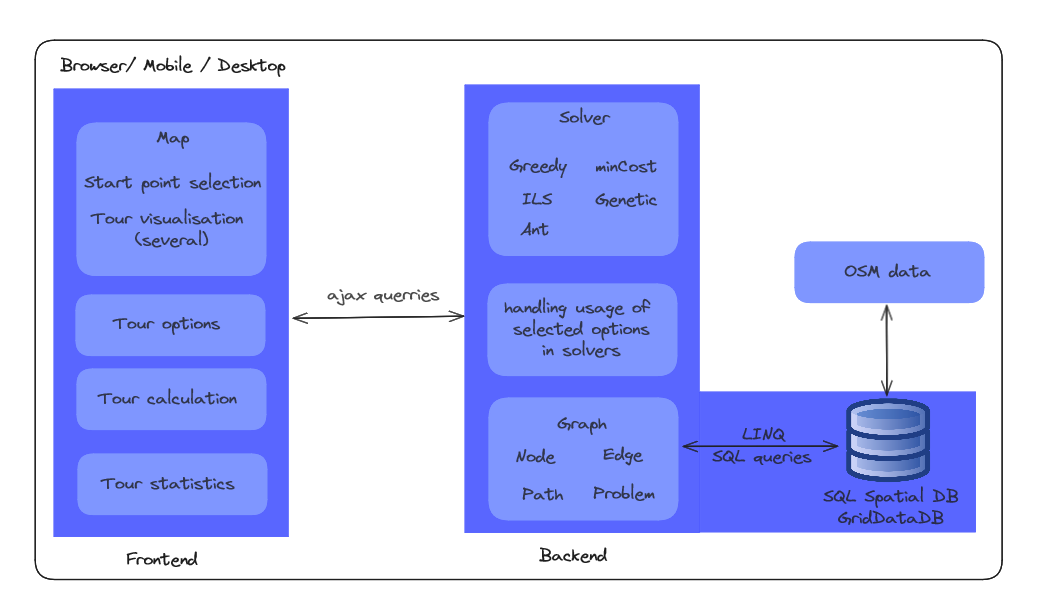
\includegraphics[width=1.1\textwidth]{bilder/Implementation Architecture.png}
	\caption{Visualization of the used architecture}
	\label{fig:architecture}
\end{figure}


In the above visualization, the whole application, the distinct parts and features as well as communications between them are illustrated. 
The front end is realized as a web application, running in the browser, but the visualization can also be customized to be executable as a mobile or desktop application (see \ref{sec:futureWork}). 
In the visualized map, the marker can be set to the current location - if the permission to access the user's location data is granted.
However, simply searching for a specific address, drag-and-dropping the marker on the map, or scrolling the map and selecting a position by clicking on the place to mark are also possible. 
Furthermore, the visualization of the calculated tours is also realized using the map and a polygon built from the respective points.
These tours can be toggled to be shown or hidden, so an easier overview is possible after generating several tours.
For debug purposes, there is a feature to show the whole graph that is being used for the calculation using the currently selected maximum length.

In addition to the main feature -- the map -- the front end also contains two menus:
One holding the parameters the user can use to customize the tours according to their preferences and the information menu containing a report of the core data of the calculated path that is being visualized. 
A more detailed description of the front end design, concept sketches and the final implementation are outlined in subsection \ref{subsec:interfaceAndFrontendChanges}.

The back end manages all solvers that have been implemented, the database objects and intermediate objects like the graph that is created from the nodes, edges and their connections. 
Furthermore the back end is responsible for handling the parameters the user chose, selecting the correct solver and generally managing the ajax requests received from the front end. 
The database objects are generated when building the graph by accessing the database and using the stored values.

Finally, the database is filled using a python script that queries OSM-data to fetch all nodes and edges for a user-selected place.
For this example, the data for Dortmund were retrieved.
In addition to the OSM data, using the latitude and longitude, elevation data are obtained from the docker server. 

\subsection{Database}
\label{subsection:database}

The database is a relational database using Microsoft SQL server, administered in Microsoft SQL Server Management Studio.
This database also allows to use spatial data, which was an important feature for storing and processing the nodes and edges.
Using the spatial features enables the possibilities to filter nodes within a given radius, retrieving only a relevant subset of data points.
This filtering option within the database significantly speeds up the data retrieval as well as the graph creation.
Compared to the previous method of generating a fixed graph for the city of Dortmund, the database offers further important advantages:
Far more nodes than only points within Dortmund can be used.
Even though the database creation and the adding of points is relatively slow, this is a process that only needs to be run once -- before the application can be used -- and does not affect the tour calculation. 
Once the data has been added, all points can be accessed without needing to retrieve the whole database.

To create the database, a python script is used. \# TODO if added, describe parameters and how to use the script with them
This script first creates an osmnx graph from OSM data using the \texttt{graph\textunderscore from\textunderscore place} function
\begin{lstlisting}
	ox.graph\textunderscore from\textunderscore place(place\textunderscore name, network\textunderscore type='all', custom\textunderscore filter=custom\textunderscore filter)
\end{lstlisting}

Here, the \texttt{place\textunderscore name} is the name of the city, state, country or region for which osmnx should gather the data points.
For a city, the city's name, state and country need to be added. 
If a whole state should be selected, the state name and country are required.
The \texttt{network\textunderscore type} has six values to choose from\footnote{\url{https://osmnx.readthedocs.io/en/stable/user-reference.html\#module-osmnx.settings}, last accessed: 19.04.2024}: \texttt{all\textunderscore private}, \texttt{all}, \texttt{bike}, \texttt{drive}, \texttt{drive\textunderscore service}, and \texttt{walk}. 

The \texttt{custom\textunderscore filter} is defined to select only those edges, where walking, running and cycling is possible by specifically de-selecting respective highway types:

\begin{lstlisting}
	custom_filter = '["highway"]["highway"!~"motorway|trunk|proposed|construction|motorway_link|trunk_link"]'
\end{lstlisting}

The excluded types are used for the following street types according to the OSM Wiki:
\begin{table}[ht]
	\centering
	\begin{tabular}{l|l}
		Highway type & Description\\
		\hline
		motorway & A restricted access major divided highway, normally with 2\\ 
		& or more running lanes plus emergency hard shoulder.\\
		& Equivalent to the Freeway, Autobahn, etc..  \\
		trunk & The most important roads in a country's system that aren't \\
		& motorways. (Need not necessarily be a divided highway.) \\
		proposed & For planned roads. \\
		construction & For roads under construction. \\
		motorway\textunderscore link & The link roads (sliproads/ramps) leading\\
		& to/from a motorway from/to a motorway or lower class highway. \\
		& Normally with the same motorway restrictions. \\
		trunk\textunderscore link & The link roads (sliproads/ramps) leading \\
		& to/from a trunk road from/to a trunk road or lower class highway. 
	\end{tabular}
	\caption[OSM highway types]{This table shows a listing of different OSM highway types and their definition taken from the Wiki page\protect\footnotemark}
	\label{tab:osmHighwayTypes}
\end{table}

\footnotetext{\url{https://wiki.openstreetmap.org/wiki/Key:highway}, last accessed: 19.04.2024}

Next, the elevation data has to be added for the nodes of this graph.
These information are not part of osmnx but need to be retrieved from a different source.
For this thesis, Open Elevation\footnote{\url{https://open-elevation.com/}, last accessed: 20.03.2024} was used.
The data were downloaded and hosted in a local docker that could be queried instead of the API.

Then, the surroundings information need to be obtained. 
These information are provided by OSM, however they are not saved for nodes.
So, a different query that retrieves areas and then matches the respective tags to the saved nodes by matching the IDs has to be executed.

After gathering all the neccessary information, the script first checks if the database already contains matching tables and if not, generates them.
Then the nodes and edges that have been retrieved from osmnx can be iterated and inserted into the database using basic SQL.
During the iteration over the edges, the references between nodes and edges can be created (inserting edges into the IncidentEdges table that manages nodes and all their incident edges as well as adding references to the source- and target node when entering the edge data).
Using these references later enables the back end code to easily access the endpoints of a graph or gather the incident edges for a node. 



\subsection{Interface and Front end changes}
\label{subsec:interfaceAndFrontendChanges}

The front end was updated from the existing version of Tour4Me to allow for a better overview after adding in several additional option for the user to select from. 
First, a conceptual idea see figures (\ref{fig:frontendConcept} to \ref{fig:frontendConceptResultsCloseup}) was built, mapping out the general structure of the new interface. 
Here, the main changes were focused on replacing the previous pop-ups through permanent menus.
On the side, a burger-menu button was added that allows for a side menu to be folded and unfolded to show the customization options (see \ref{fig:frontendSideMenuCloseups}). 
The result view was moved from an overlay on the map to a foldable footer menu (\ref{fig:frontendConceptResultsCloseup}). 
Furthermore, the displayed tours and the respective information can now be unfolded additionally in this footer menu.
Previously, the tour information (including the length and other relevant data) was only accessible through a popup. 

Displaying all the resulting data while giving the option to fold and unfold them allows the user easier access as well as enables easier comparison between different tours.
Previously, only the data of a single tour could be shown in the popup. 
Now, the information of all tours are visible at the same time. 



\# TODO move this to the appendix maybe?
\begin{figure}[H]
	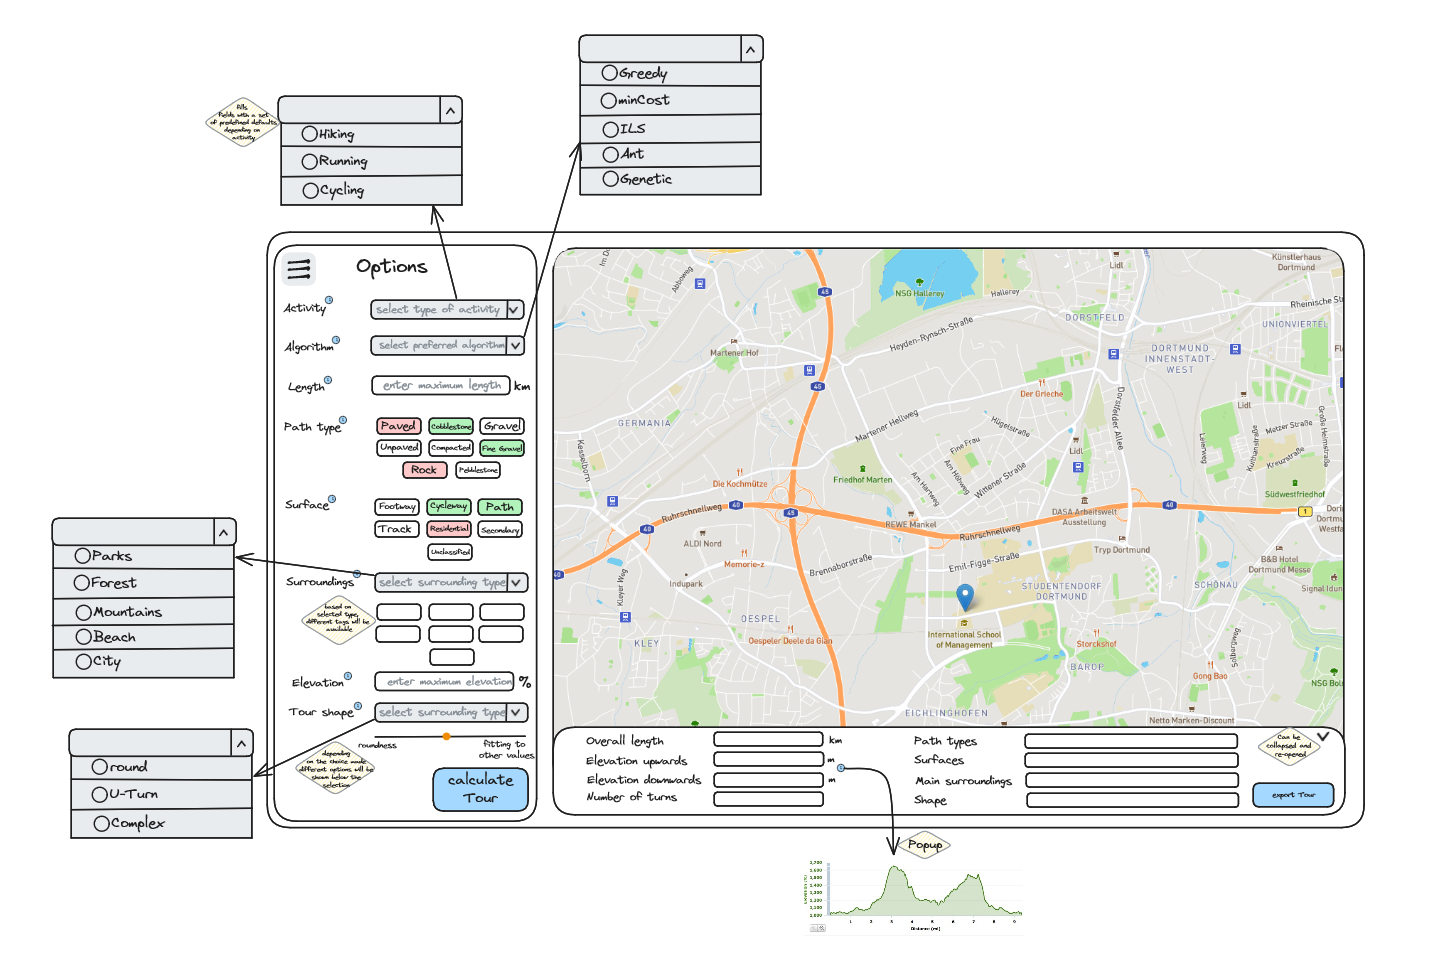
\includegraphics[width=0.9\linewidth]{bilder/Concept new Frontend design.png}
	\caption{Design concept for the front end view, including descriptions for drop-downs and pop-ups}
	\label{fig:frontendConcept}
\end{figure}



The new interface now has a more botanic color scheme, using mainly dark greens, browns and blue while the text is off-white.
The side menu \textit{options} displays a wider selection of preference settings.
In figure \ref{fig:actualFrontendSideMenu}, the side menu is visualized. 
The uppermost drop down (see \ref{fig:actualFrontendSideMenuActivity}) can be used to set a pre-selection that fills in the following fields with suggested default values. 
These values can always be customized afterwards, but could offer a higher usability.
The next selection shows all currently implemented algorithms (see \ref{fig:actualFrontendSideMenuAlgorithm}).
Depending on the choice, the results will turn out differently.
While greedy always only prioritizes the maximum edge profit and ignores the roundness of the tour, MinCost does the exact opposite.
AntColony is more focused on edge profit, but also takes elevation and roundness into account.
And finally simulated annealing produces results that are mostly focused on roundness while still taking edge profits and elevation into consideration. 
The respective combinations start with greedy or MinCost and then strive to improve them. 

All following options are direct tour parameters and describe user preferences.
The length is an estimate of the final tour length, that is never used as a hard stop but allows for tours to be within a range of a few hundred meters longer or shorter than the selected length.
However, tours are never more than a kilometer longer or shorter than the selected length.
\# TODO check that this is true lol


Surface and path type show selection buttons.
These buttons can be neutral (when they only show a white border), positive (colored in green) or negative (colored in red). 
A neutral button describes properties that are neither preferable nor undesirable while green marks preferred values and red marks undesirable values.
Surfaces describe properties of the ground, path types characterize the type of street.
In OSM, there are many other options, however some are already filtered (for example highways) and others are not of much interest and would only result in an overwhelmingly large selection.
Surroundings have a drop down menu to select a general type -- the forest, grasslands or other options -- that will then display the respective tags to display (see \ref{fig:actualFrontendSideMenuSurroundings}). 
This approach was used to minimize the number of tags and allow for an easier overview for the user.

The tour shape offers the options to pick a round tour, a U-turn, a complex tour or do a custom selection (see \ref{fig:actualFrontendSideMenuTourShape}). 
Round tours have the highest importance (80 \%)on the roundness of a tour and split the remaining 20\% between elevation and edge profits. 
This makes rounder tours more likely to be calculated.
U-turns can have a special implementation that ensures for a slightly different path back to the beginning, but currently simply levels the importance of edge profits and elevation while ignoring the covered area.
Complex tours are similar, but don't fully remove the importance of the area. 
For the custom selection, three sliders are displayed.
These slider inputs are linked so they influence each other, ensuring that the three probabilities always sum to 100\%.

Below the tour shape, elevation and steepness can be selected. 
The elevation describes the maximum difference in elevation for the whole tour. 
This property does not differentiate between ascending or descending parts but sums up all differences and divides the overall result by two, to accommodate for the roundtrip. 
The steepness is used to exclude any part of the tour from being steeper than the chosen limit as much as possible.
With the inaccuracy of the elevation data, this can sometimes be impossible.
In these cases, creating any tour, even if it exceeds the limit is seen as more desirable than having no result at all.

At the bottom, the maximum runtime can be chosen, however no algorithm runs as long as 30 seconds with the current settings.
Clicking the button \glqq Compute Path\grqq{} will then trigger a query to the back end, where all the selected information are processed, the matching solver is selected and a tour is calculated.
The resulting roundtrip is then parsed into the latitude and longitude values of the nodes that form the tour and returned to the front end.
Here, the latitude and longitude values can then be displayed and connected to form a polygon that visualizes the resulting tour.

\begin{figure}[H]
	\centering
	\sbox{\measurebox}{%
		\begin{minipage}[b]{.25\textwidth}
			\subfloat
			[]
			{\label{fig:actualFrontendFullSideMenu}\includegraphics[height=0.5\textheight]{bilder/actualFrontendSideMenu.png}}
	\end{minipage}}
	\usebox{\measurebox}\qquad\hfill
	\begin{minipage}[b][\ht\measurebox][s]{.5\textwidth}
		\centering
		\subfloat
		[]
		{\label{fig:actualFrontendSurroundignsForest}\includegraphics[width=0.9\textwidth]{bilder/actualFrontendSideMenuSurroundingsForestSelected.png}}
		
		\vfill
		
		\subfloat
		[]
		{\label{fig:actualFrontendTourShapeCustomSliders}\includegraphics[width=0.9\textwidth]{bilder/actualFrontendSideMenuTourShapeCustomAndSlider.png}}
	\end{minipage}
	\caption{This figure shows the newly implemented side menu. (a) displays the full side menu (b) is a closeup of the surroundings when \textit{forest} is selected and (c) shows the three importance sliders when the selected tour shape is \textit{custom}}
	\label{fig:actualFrontendSideMenu}
\end{figure}

All additional information are displayed in the \textit{Route information} footer menu. 
The menu as well as the calculated tours can be folded and unfolded.
This option does not decrease the size of the map but rather results in an added scroll-option, so the additional information can be displayed below the map.
The shown tours are colored in the same color as the respective displayed tour. 
A selection of ten colors is implemented, allowing for ten different tours to be calculated and displayed before a color is repeated. 
All of these colors are kept within the same botanical color scheme.
Next to the tour name, the used algorithm is written.
Furthermore, there are two buttons to toggle the visibility of the polyline in the leaflet map or to delete the generated tour entirely.

\begin{figure}[H]
	\centering
	\includegraphics[width=0.9\textwidth]{bilder/routeInformationOneTour.png}
	\caption{This shows the Route information menu with one tour and all the related information unfolded and displayed}
	\label{fig:actualFrontendToureInfoMenuOneTour}
\end{figure}

Clicking on the tour name will fold (see \ref{fig:actualFrontendToureInfoMenuMoreTours}) and unfold (see \ref{fig:actualFrontendToureInfoMenuOneTour}) the respective information.
In this view, the final overall length, elevation, maximum steepness, collected Edge profits, total quality, covered area and for reference the maximum possible covered area given the same extreme points as the current tour has.
On the right side, the collected path types and surfaces, surroundings and the time it took to initialize the graph and to calculate the tour as well as the memory consumption are displayed.
The last three values are not as interesting for the typical user but allow for a deeper insight into the calculation. 
Removing the outputs for a final version is easily done if needed. 



\begin{figure}[H]
	\centering
	\includegraphics[width=0.5\textwidth]{bilder/routeInformationMoreTours.png}
	\caption{This shows the Route information menu with several folded tours displayed}
	\label{fig:actualFrontendToureInfoMenuMoreTours}
\end{figure}


\section{Algorithmic changes}
\label{sec:algorithmicChanges}

\subsection{Ant Colony}
\label{subsec:antColonyImplementation}


\subsection{Simulated Annealing}
\label{subsec:simulatedAnnealingImplementation}




The quality of the solution is calculated based on the covered area A and the respective importance (areaImportance), the edge profit (P) and the respective importance (edgeImportance) and all other valuable properties (others) and scaled by the target length of the tour (L). 

\begin{equation}\label{eq:qualitySA}
	f(i) = \frac{areaImportance * A(i)}{\pi * L(i)^2} + \frac{edgeImportance * P(i)}{L(i)} + others(i)
\end{equation}


\section{Parameter changes}
\label{sec:parameterChanges}

